\documentclass{article}
\usepackage[T1]{fontenc}
\usepackage{microtype,booktabs,xurl}
\usepackage{tikz,pgfplots}
\usetikzlibrary{arrows.meta,positioning}
\pgfplotsset{compat=1.18}
\usepackage[hyperfootnotes=false]{hyperref}
\usepackage{mlsys2025}
\hypersetup{hypertexnames=false}
\mlsystitlerunning{From Resource Savings to Useful Answers: Artifact Appendix}
\begin{document}
\twocolumn[
\mlsystitle{From Resource Savings to Useful Answers:\\Separate Artifact and Evidence Appendix}
\begin{mlsysauthorlist}
\mlsysauthor{Anonymous Authors}{anon}
\end{mlsysauthorlist}
\mlsysaffiliation{anon}{Anonymous Institution}
\mlsyscorrespondingauthor{Anonymous Author}{anon.email@domain.com}
\vskip .3in
]
\appendix
\section{Evidence Lineages and Scope}
The main manuscript separates historical accounting/precision protocols,
four-node release/state validation, and single-node execution/application
experiments. A report's existence does not make its scope interchangeable with
another. The artifact separates recorded findings from new reproduction runs. No
artifact badge or independent reproduction is claimed.
No command below deploys a pod or starts a new experiment.

The final single-node reports are copied unchanged to
\path{evidence/2026-10-24-final/prefill.json} and
\path{evidence/2026-10-24-final/validation.json}.
Their source SHA256 digests, derived cells and application summaries are in
\path{generated/derived.json}. Both report completed status. The first contains
112 execution cells; the second 36 old-fixture evaluation cells, 72 new-document
cells and 12 application episodes. The 24 application answer generations are
stored within those episodes, not counted as independent new-document samples.

Earlier running-campaign snapshots and previous manuscript versions remain
historical source archives. They are not new scientific runs and are not
bundled with this release; the current figures use the final reports.

\section{Read-Only Figure and Table Verification}
From the paper directory, run
\begin{quote}
\texttt{python3}\\
\path{build_research_evidence.py}
\end{quote}
The default audits source completion/counts, completed evaluation cells with three runs,
per-case quality outcomes and derived medians. It verifies all TeX table rows,
prefix/latency data and measured timeline coordinates. Explicit
\texttt{--write} regenerates derived files from the same frozen sources.
No smoothing, selected confidence interval or generated example result is used.

The quality matrix reorders original cohort indices into answerable then
unanswerable halves, preserving source order within each. Green follows the
original automatic pass. Amber is a post-hoc diagnostic requiring an
unanswerable question, failed contract and output beginning with unknown;
it does not reclassify a failure or adjudicate semantic correctness. Gray
contains the other automatic failures. The episode timeline uses block 1 of
all four policies, chosen by fixed cohort order, not best outcome; it is not
composed from policy-wise medians. The fresh inference bar begins at measured
fresh completion minus its measured request duration.

\section{Method Pins and Failure Accounting}
The standard server and private prototype use frozen runtime revision
\path{838374375cb8c467c33c263be4801c19d1089763} with separate source/binary manifests.
Full model SHA256 is
\path{8123a526b3c9b9eeda6cb1dd3af78bd1de0da9af2cef8259f52c3e0a8cd3cebd}.
Context is 2048, greedy cap 64, no GPU. The baseline compares raw KV-F32 batches
64/256/512 and batch512 KV-F16/flash-auto, repacking enabled, 4/2 phase threads,
logical batch512, one slot. The prototype fixes logical frame64, repack64,
KV-F32 and optional attention mask39--42. Prompt reuse is disabled in both.
In this server, final \texttt{tokens\_cached} is slot occupancy; actual reuse is
checked using \texttt{timings.cache\_n} and processed prompt count.

A missing standard shared library caused an initial deployment to stop before
model loading. No rows from that attempt enter the reported run. The corrected
package passed an ARM executable check; source/config hashes were frozen again.
The earlier CoQA cohort preparation did not supply enough conservatively
eligible records; SQuAD2 was selected prospectively before its inference. These
are preparation failures, not hidden task exclusions after observing answers.

Memory reports distinguish RSS, anonymous/file pages, PSS and node availability.
VmHWM is process-lifetime and cgroup peak pod-lifetime. Page-charge ownership is
not reassigned; 12 GiB is a safety cap. Model startup is separated by readiness,
while warm requests always clear KV. No energy measurement is supplied.

\section{New-Document Evaluation and Human Review}
The official SQuAD2 development JSON SHA256 is
\path{80a5225e94905956a6446d296ca1093975c4d3b3260f1d6c8f68bc2ab77182d8};
the evaluator SHA256 is
\path{710840ce2c2c61716334c056777032f24660b83eb9869a451036e6a24d8103c4}.
Data use follows the project's CC BY-SA attribution. Raw selected contexts,
reference alternatives, questions and exposure audit are preserved locally;
no model-training cleanliness or unrestricted redistribution is implied.

Selection fixes 24 distinct article titles, one question each, alternating 12
answerable/12 unanswerable cases, input at most 1200 tokens. Prior exposure
checks exact quoted SQuAD question IDs in the listed JSON records and exact
normalized CoQA story duplication; unlogged use and paraphrase overlap remain
possible. Mean F1/EM use official reference matching after removing parsed
citations. Bare unknown maps to the official empty-answer representation for
unanswerable cases. No confidence threshold is tuned. Exact-reference agreement,
EOS and a valid locator define the frozen proxy, not independent semantics.

The artifact retains ordinary and blinded answer-review JSONL packets plus a
separate arm/metric key. Source, question, reference spans and generated strings
are available to a reviewer without intervention labels in the blinded version.
Human correctness/support fields remain null. The manuscript's qualitative
interpretation is explicitly unblinded AI-assisted inspection.

\section{Application Reproduction Boundary}
Each matched block adds a different new source to the same real incremental
Git update; all policies receive identical snapshots for that block. Three
blocks are not within-document replications. v1 is constructed before timing;
the new source must be absent. Encoder batch4, intra-op2/inter-op1, stable
chunks at most 256 tokens are fixed. The current request uses pinned old oracle
evidence; only the fresh request performs actual v2 dense-top3 retrieval.
The same clock origin measures current completion, publication and fresh
completion. Publication is observed when the publisher returns, not a claimed
hardware-level commit timestamp. Citation checks require locators present in
the returned passages. Failed episodes remain represented in the timing table.

All-episode checks fail because the third fresh answer elaborates a reference
phrase, and one full-prototype answer has a malformed citation prefix. Frozen
verdicts remain unchanged. A future human assessment is separate evidence, not
an overwrite of automatic scores. There is no justified service SLA, weighted
utility score, significance test or automatically scheduled distributed extension.

\section{Artifact Coverage and Historical Context}
The artifact covers the Qwen2.5-14B experiments reported in the main paper:
distributed precision and KV controls, decode-overlap ingestion, native
prefill and attention omission, standard-backend and new-document evaluation,
sequential application controls and E1--E3. Its coverage table connects each
finding to code, fixed inputs, recorded evidence and a rerun command.

Earlier TinyLlama A/P0/C protocols are separate historical context. Their
results are not pooled into this Qwen study, and the release does not include
unrelated local archives. The native release records are bundled under
\path{evidence/distributed/}, relative to the artifact root. Compressed
full-logit matrices support recomputation of the twelve quality jobs. The
original teacher-forced and generated passes remain distinct from application
request latency.

\section{Build and Availability}
Build each PDF using \texttt{latexmk -pdf -interaction=nonstopmode -halt-on-error}
followed by \texttt{main.tex} or \texttt{artifact-appendix.tex}. Official style,
font sizes and margins are unmodified. The dedicated artifact branch includes
native and Python source, deployment definitions, fixed inputs and a read-only
evidence audit. The root \path{ARTIFACT.md} describes setup and validation.
A fresh complete ARM64 campaign and exact model regeneration remain to be
validated for this portable release. No badge or independent reproduction
claim follows from build and software checks.
\section{E1--E3 Evaluation Evidence}
The additional 27 diagnostic cells, 36 independent-arrival application episodes
and 12 timing-holdout episodes are frozen separately under
\path{evidence/2026-10-27/}. Files \path{e1.json}, \path{e2.json} and
\path{e3.json} retain complete reports. \path{predictions.json} retains the
prelaunch prediction freeze; \path{audit.json} records source digests and
post-hoc numerical diagnostics. Run \path{build_budget_evidence.py} with Python3
to verify the reports, counts, prediction digest and generated phase figure.
The main text's earlier controls remain a separate lineage.

E2 contains 17 recovered and 19 continuation episodes after a documented
sampler failure; no completed episode was repeated. Symlinks are retained in
collection archives without dereferencing. The artifact cross-stage audit additionally checks the 37,475 bundled
affinity samples and original-prefix integrity.
The constant-policy prediction baseline was added after E3 as a diagnostic,
not as a frozen confirmatory comparison. No predictor was refitted. All E3
cases remain slot limited; answer-level semantic adjudication is pending.

\section{Earlier Distributed Release Lifecycle}

The native transition worker operates on stage 0 of a four-stage Qwen2.5-14B
route. Each stage contains 12 transformer layers; the other stages keep Q4
weights. Q4/Q3 mean Q4\_K\_M/Q3\_K\_M mixed GGUF formats, not uniformly
four-/three-bit tensors. Target shards are prepositioned and hash-checked;
network installation is outside this pilot.

At a token boundary, the coordinator pauses issuance, exports stage KV,
destroys the executor and unmaps the old shard before mapping the target.
The worker constructs the target executor, imports state and verifies a
re-export for byte and metadata equality. A replacement failure stops execution;
there is no rollback or zero-downtime guarantee. Serialized KV and runtime
allocations remain temporary costs, and unmapping does not evict shared page
cache. The same path restores Q4. Same-precision controls test transfer integrity.
\begin{figure}[t]
\centering
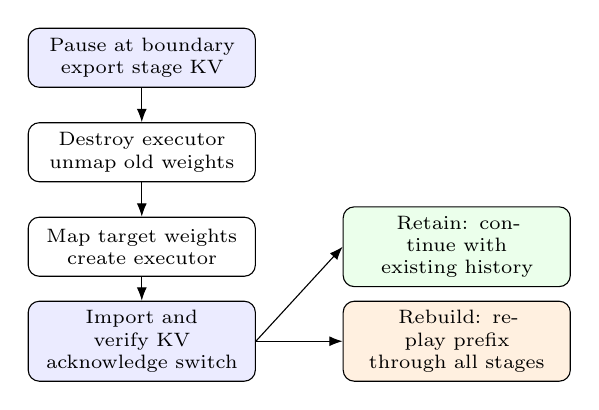
\begin{tikzpicture}[font=\scriptsize,box/.style={draw,rounded corners,align=center,text width=2.65cm,minimum height=.75cm},>=Latex]
\node[box,fill=blue!8] (a) at (0,0) {Pause at boundary\\export stage KV};
\node[box] (b) at (0,-1.2) {Destroy executor\\unmap old weights};
\node[box] (c) at (0,-2.4) {Map target weights\\create executor};
\node[box,fill=blue!8] (d) at (0,-3.6) {Import and verify KV\\acknowledge switch};
\node[box,fill=green!8] (e) at (4,-2.4) {Retain: continue with\\existing history};
\node[box,fill=orange!12] (f) at (4,-3.6) {Rebuild: replay prefix\\through all stages};
\draw[->] (a)--(b);\draw[->] (b)--(c);\draw[->] (c)--(d);
\draw[->] (d.east)--(e.west);\draw[->] (d)--(f);
\end{tikzpicture}
\caption{Implemented switch lifecycle. Old weights are unmapped before target
mapping. KV export still needs temporary memory. Import integrity is distinct
from target-model fidelity. Failure stops the worker; there is no rollback.}
\label{fig:lifecycle}
\end{figure}


Retention continues with the existing history. Rebuilding instead clears and
replays the prefix through \emph{all four stages}: unchanged downstream weights
can still have state derived from changed upstream activations. Import equality
therefore checks serialization, not equivalence to state recomputed at the
target precision. Full replay is a control, not a new selective-repair method.


\begin{figure}[t]
\centering
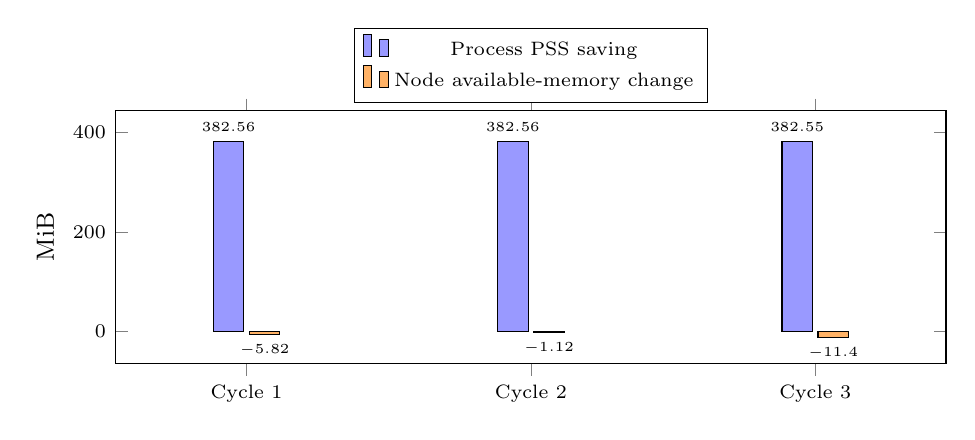
\begin{tikzpicture}
\begin{axis}[width=\columnwidth,height=4.8cm,ybar,bar width=11pt,ymin=-65,ymax=445,
 ylabel={MiB},symbolic x coords={Cycle 1,Cycle 2,Cycle 3},xtick=data,
 tick label style={font=\scriptsize},label style={font=\small},
 legend style={font=\scriptsize,at={(.5,1.03)},anchor=south,legend columns=1},
 nodes near coords,nodes near coords style={font=\tiny},enlarge x limits=.23]
\addplot[fill=blue!40] coordinates {(Cycle 1,382.56) (Cycle 2,382.56) (Cycle 3,382.55)};
\addplot[fill=orange!60] coordinates {(Cycle 1,-5.82) (Cycle 2,-1.12) (Cycle 3,-11.40)};
\legend{Process PSS saving,Node available-memory change}
\end{axis}
\end{tikzpicture}
\caption{Paired warmed Q4-to-Q3 observations. Positive PSS saving means a
smaller process footprint. Node availability does not increase in any cycle.
These metrics are not interchangeable or additive.}\label{fig:memory}
\end{figure}

\end{document}
